
\chapter{GAs: Experimental Results and Limitations}
\label{GAs_experiment}

While numerous fitness functions, hyperparameters, and QUBO instances were experimented with and validated during the research phase, this section reports the most prominent results to highlight the critical operational aspects in using Genetic Algorithm with our embedding architecture. 

\section{Validation on a 5x5 Instance}

To rigorously validate the embedding model, the experimental phase was initiated with a relatively small-scale $5 \times 5$ instance, as depicted in Figure \ref{fig:5x5_qubo_instance}.

\begin{figure}[htbp]
    \centering
    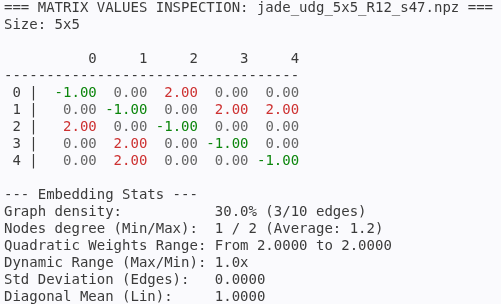
\includegraphics[width=0.6\textwidth]{img/QUBO_instances/5x5_UDG_r12_s47.png} 
    \caption{Structure of the small-scale UDG-like QUBO instance ($N=5$) generated via \textit{instance\_generator.py}, inspected using \textit{inspect\_qubo.py}, and subsequently embedded using the \textit{bench-GA.py} module \cite{orsucci_qubo_ga_quantum}.}
    \label{fig:5x5_qubo_instance}
\end{figure}

This specific configuration serves as an ideal baseline candidate. Despite its small dimensionality, it features a non-trivial density and a mathematically interesting topology composed of disconnected sub-graphs: a two-node island connecting $q_0$ and $q_2$, and a separate localized chain linking $q_1$, $q_3$, and $q_4$.

The Genetic Algorithm was executed utilizing a multi-start approach consisting of 5 independent runs. This specific volume of restarts was empirically established as an optimal trade-off between maximizing the probability of finding the global spatial optimum and maintaining a manageable classical execution time, thereby mitigating the inherent stochastic nature of evolutionary algorithms. The hyperparameters employed for this specific dimensional scale are detailed in Table \ref{tab:pygad_parameters}.

\begin{table}[htbp]
    \centering
    \renewcommand{\arraystretch}{1.3}
    \resizebox{\textwidth}{!}{
    \begin{tabular}{l c p{0.55\textwidth}}
        \hline
        \textbf{PyGAD Parameter} & \textbf{Configured Value} & \textbf{Conceptual Meaning} \\
        \hline
        \texttt{num\_genes} & $2 \times N_{atoms}$ & Chromosome length: represents continuous 2D coordinates $(x,y)$ for all atoms. \\
        \texttt{sol\_per\_pop} & $100$ & Population size: number of candidate physical layouts per generation. \\
        \texttt{num\_generations} & $800$ & Termination criterion for the evolutionary loop. \\
        \texttt{fitness\_func} & \texttt{improved\_topological\_MAE} & Custom evaluation metric (incorporates topological error and hardware physical penalties). \\
        \texttt{parent\_selection\_type} & Tournament & Selection strategy to maintain competitive evolutionary pressure. \\
        \texttt{K\_tournament} & $3$ & Number of candidate individuals competing in each selection tournament. \\
        \texttt{num\_parents\_mating} & $20$ & Number of parents successfully selected to compose the mating pool. \\
        \texttt{crossover\_type} & Uniform & Exchanges individual $(x,y)$ coordinates between parents without disrupting array bounds. \\
        \texttt{mutation\_type} & Adaptive & Dynamically scales mutation rate to balance exploration and fine-tuning. \\
        \texttt{mutation\_probability} & $[0.4, 0.05]$ & Assigns a $40\%$ mutation rate to low-fitness individuals and $5\%$ to elite ones. \\
        \texttt{random\_mutation\_min/max} & $[-3.0, 3.0]$ & Continuous spatial perturbation window (in $\mu$m) for local coordinate adjustments. \\
        \texttt{keep\_elitism} & $5$ & Preserves the absolute best $5$ layouts across generations without any genetic alteration. \\
        \texttt{allow\_duplicate\_genes} & False & Prevents multiple atoms from collapsing into the exact same mathematical coordinates. \\
        \hline
    \end{tabular}
    }
    \caption{Exact hyperparameter configuration adopted for the Genetic Algorithm setup using the PyGAD library, referencing the base architecture for a $5 \times 5$ problem embedding.}
    \label{tab:pygad_parameters}
\end{table}

As evident from the table, the parametrization is not excessively aggressive. Because the spatial search space for a 5-node matrix is relatively contained, extremely high mutation parameters are not required to avoid local minima. Under this configuration, the best evolutionary run achieved an excellent spatial fitness score of $0.3968$, demanding a total classical CPU execution time of $144.35$ seconds. Most importantly, this run generated the geometrically feasible embedding illustrated in Figure \ref{fig:5x5_register}.

\begin{figure}[htbp]
    \centering
    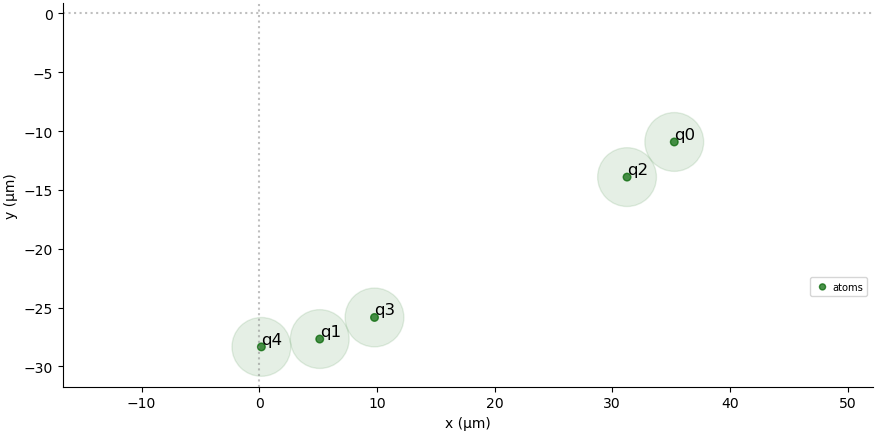
\includegraphics[width=0.8\textwidth]{img/embedding/reg_5x5.png} 
    \caption{The 2D physical spatial layout generated by the Genetic Algorithm for the $N=5$ instance. The register fully complies with Neutral Atom QPU geometric boundaries.}
    \label{fig:5x5_register}
\end{figure}

The physical layout intuitively respects the mathematical constraints previously analyzed, properly isolating the distinct logical islands while strictly adhering to the minimum inter-atomic distance and maximum global radius imposed by the hardware profile. When these physical coordinates were compiled into an adiabatic sequence and submitted to the QPU emulator, the system produced the output distribution shown in Figure \ref{fig:5x5_quantum_res}.

\begin{figure}[htbp]
    \centering
    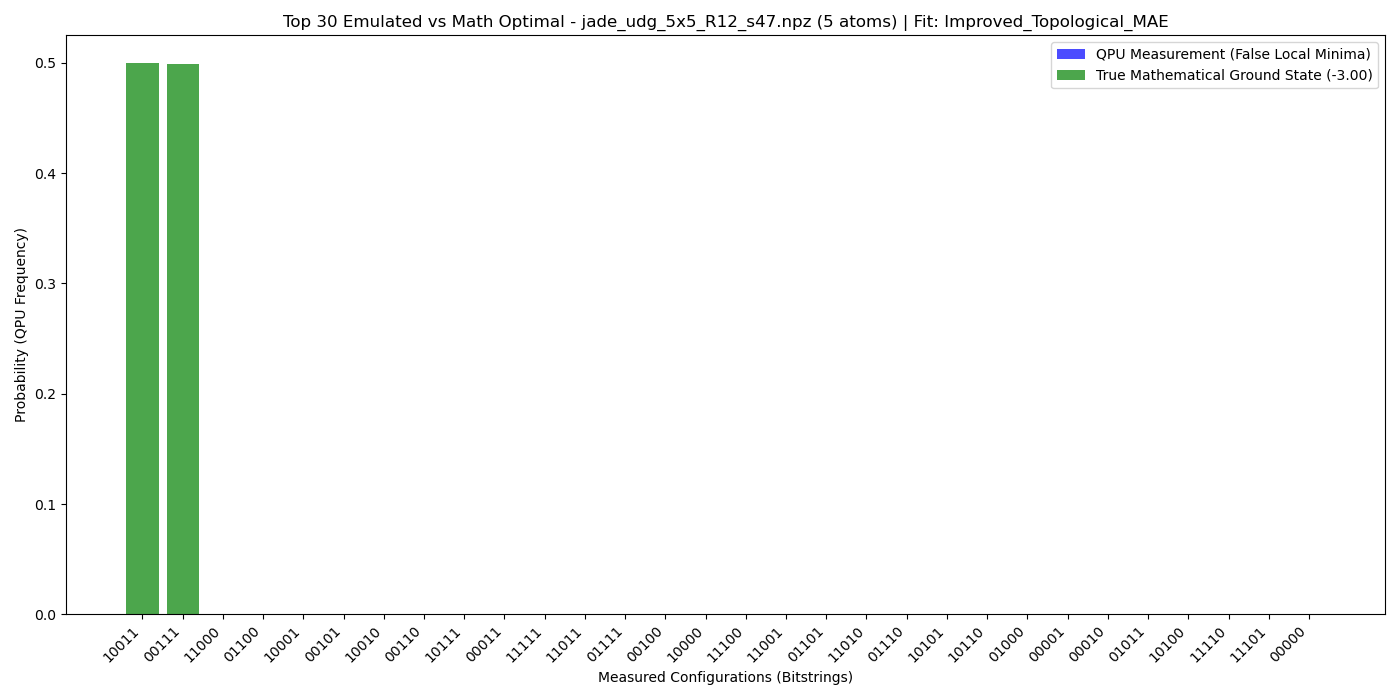
\includegraphics[width=1.0\textwidth]{img/res/res_5x5.png} 
    \caption{Probability distribution of the measured bitstrings after the adiabatic execution on the QPU emulator. The highest probability peaks correspond perfectly to the optimal solutions of the original QUBO instance.}
    \label{fig:5x5_quantum_res}
\end{figure}

The quantum execution demonstrates outstanding performance: the analog platform identified the two optimal ground states found with classical brute-force method (suitable for small instances like in this case) with exceptionally high probability and symmetry. This initial validation serves as a highly encouraging proof-of-concept for our hybrid pipeline, setting the baseline to systematically investigate the scalability limits of this exact mathematical approach.
\section{Scaling Validation on a 6x6 Instance}

Continuing the systematic scaling tests, the problem dimensionality was incrementally increased. For the $6 \times 6$ dimensional scale, the target matrix is depicted in Figure \ref{fig:6x6_qubo_instance}.

\begin{figure}[htbp]
    \centering
    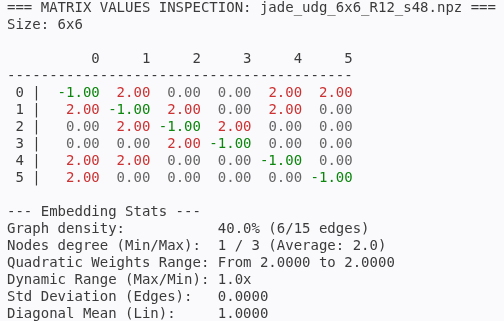
\includegraphics[width=0.6\textwidth]{img/QUBO_instances/6x6_UDG_r12_s48.png} 
    \caption{Structure of the $6 \times 6$ UDG-like QUBO instance generated via \textit{instance\_generator.py}, inspected using \textit{inspect\_qubo.py}, and subsequently embedded using the \textit{bench-GA.py} module \cite{orsucci_qubo_ga_quantum}.}
    \label{fig:6x6_qubo_instance}
\end{figure}

This specific configuration presents an increased graph density and a maximum node degree of $3$, introducing topological constraints that are significantly less trivial than those encountered in the $5 \times 5$ instance. To properly explore the vastly expanded continuous search space and prevent premature convergence, the Genetic Algorithm's hyperparameters required a more aggressive tuning, as detailed in Table \ref{tab:pygad_boosted_parameters}.

\begin{table}[htbp]
    \centering
    \renewcommand{\arraystretch}{1.2}
    \resizebox{\textwidth}{!}{
    \begin{tabular}{l c p{0.6\textwidth}}
        \hline
        \textbf{PyGAD Parameter} & \textbf{Updated Value} & \textbf{Conceptual Meaning} \\
        \hline
        \texttt{sol\_per\_pop} & $200$ & Population size doubled (from $100$) to enhance genetic diversity and broaden the exploration capabilities within a vaster search space. \\
        \texttt{num\_generations} & $1500$ & Increased termination limit (from $800$) to grant the evolutionary engine sufficient time to converge on harder topologies. \\
        \texttt{fitness\_func} & \texttt{improved\_topological\_MAE} & Transitioned to the refined metric (handling potential clipping and inactive bounds penalties) to better guide complex layouts. \\
        \hline
    \end{tabular}
    }
    \caption{Boosted hyperparameter configuration for more complex QUBO instances. All other evolutionary operators and parameters not explicitly listed here remain strictly identical to the baseline configuration previously defined in Table \ref{tab:pygad_parameters}.}
    \label{tab:pygad_boosted_parameters}
\end{table}

To further compensate for the structural difficulty of the matrix, the number of independent algorithm restarts was increased to 10. Under these constrained conditions, the best spatial embedding achieved is shown in Figure \ref{fig:6x6_register}.

\begin{figure}[htbp]
    \centering
    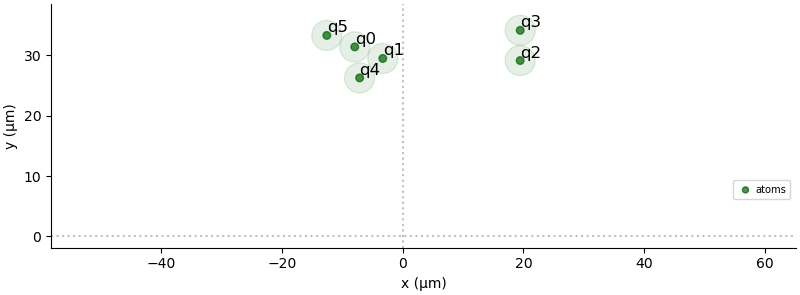
\includegraphics[width=0.8\textwidth]{img/embedding/reg_6x6.png} 
    \caption{The 2D physical spatial layout generated by the Genetic Algorithm for the $N=6$ instance. The register fully complies with Neutral Atom QPU geometric boundaries.}
    \label{fig:6x6_register}
\end{figure}

This configuration yielded a relatively low best spatial fitness score of $0.0136$, demanding a classical computational execution time of $1176.26$ seconds. When submitted to the analog emulator, the quantum execution produced the measurement distribution reported in Figure \ref{fig:6x6_quantum_res}.

\begin{figure}[htbp]
    \centering
    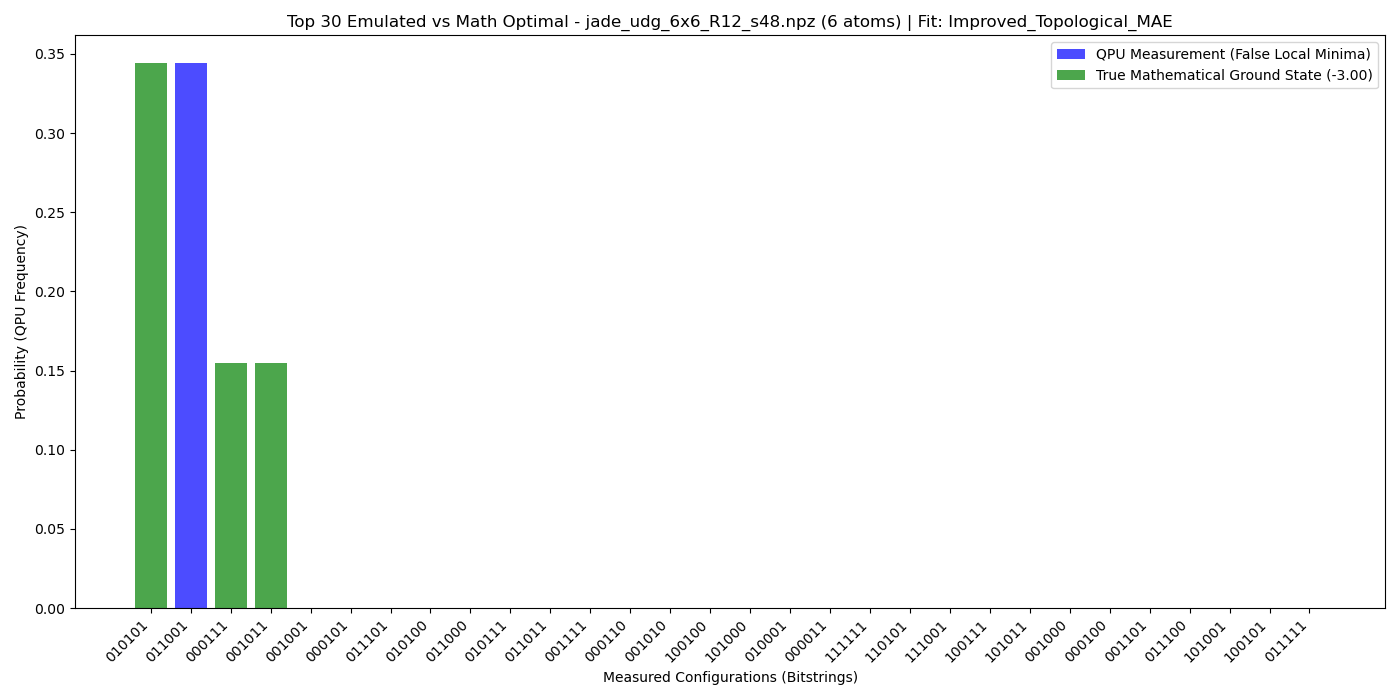
\includegraphics[width=1.0\textwidth]{img/res/res_6x6.png} 
    \caption{Probability distribution of the measured bitstrings after the adiabatic execution. Unlike the smaller instance, the highest probability peak corresponds to a false local minimum, while the true mathematical optimal solutions retain a lower, yet sufficient, cumulative probability mass.}
    \label{fig:6x6_quantum_res}
\end{figure}

Analyzing the probability distribution, a critical phenomenon emerges: the highest probability peak no longer corresponds to the true mathematical ground state, but rather to an excited state (a false local minimum). However, the true optimal solutions are still identified with a sufficiently high cumulative probability mass. Since quantum computation ultimately relies on statistical sampling, successfully isolating the optimal energy solution among the measured bitstrings constitutes a valid problem resolution.

Crucially, this result highlights the \textit{analog resilience} of the Neutral Atom QPU. It demonstrates that finding a mathematically "perfect" embedding is not strictly necessary; a "good enough" layout (even with a low fitness score of $0.0136$) can still guide the quantum dynamics toward the global optimum with an acceptable degree of success. 

While the classical execution time required to compute this embedding ($\sim 20$ minutes) is substantial, it must be contextualized. Firstly, it heavily depends on the consumer-grade hardware utilized for the preprocessing phase (refer to Appendix \ref{app:hardware_specs} for local hardware specifications). Secondly, at this preliminary stage of the research, the primary objective is validating the physical capability of the architecture rather than optimizing its classical runtime overhead.

\section{Scaling Analysis: A 7x7 Instance}

This specific instance is presented to highlight an interesting consideration regarding problem difficulty and embedding complexity. The mathematical formulation of the target problem is shown in Figure \ref{fig:7x7_qubo_instance}.

\begin{figure}[htbp]
    \centering
    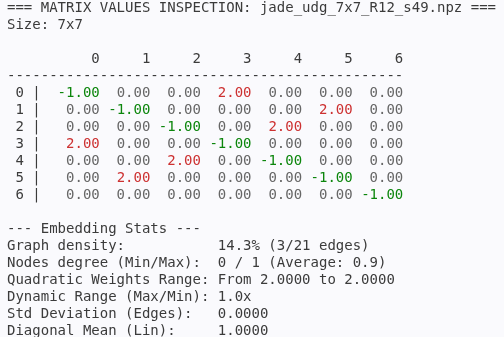
\includegraphics[width=0.6\textwidth]{img/QUBO_instances/7x7_UDG_r12_s49.png} 
    \caption{Structure of the $7 \times 7$ UDG-like QUBO instance generated via \textit{instance\_generator.py}, inspected using \textit{inspect\_qubo.py}, and subsequently embedded using the \textit{bench-GA.py} module \cite{orsucci_qubo_ga_quantum}.}
    \label{fig:7x7_qubo_instance}
\end{figure}

It is important to note that while a larger number of nodes typically implies a higher spatial embedding difficulty, this specific matrix exhibits a lower graph density and a reduced maximum node degree compared to the previous $6 \times 6$ instance. As will be demonstrated, these specific topological traits significantly facilitate the algorithmic layout process.

Consequently, despite the increased dimensionality, the Genetic Algorithm was executed using a less aggressive configuration, altering only a single parameter compared to the baseline $5 \times 5$ setup, as detailed in Table \ref{tab:pygad_reverted_parameters}.

\begin{table}[htbp]
    \centering
    \renewcommand{\arraystretch}{1.3}
    \resizebox{\textwidth}{!}{
    \begin{tabular}{l c p{0.6\textwidth}}
        \hline
        \textbf{PyGAD Parameter} & \textbf{Updated Value} & \textbf{Conceptual Meaning} \\
        \hline
        \texttt{fitness\_func} & \texttt{improved\_topological\_MAE} & Retained the refined metric (handling complex bounds and hardware penalties) to guide the layout effectively. \\
        \hline
    \end{tabular}
    }
    \caption{Hyperparameter configuration for further scaling tests. To isolate the impact of the evaluation metric and optimize classical execution times, the population size and generation limits were reverted to their original baseline values ($100$ and $800$, respectively, as in Table \ref{tab:pygad_parameters}.}
    \label{tab:pygad_reverted_parameters}
\end{table}

Executing the algorithm under these parameters yielded the spatial embedding illustrated in Figure \ref{fig:7x7_register}.

\begin{figure}[htbp]
    \centering
    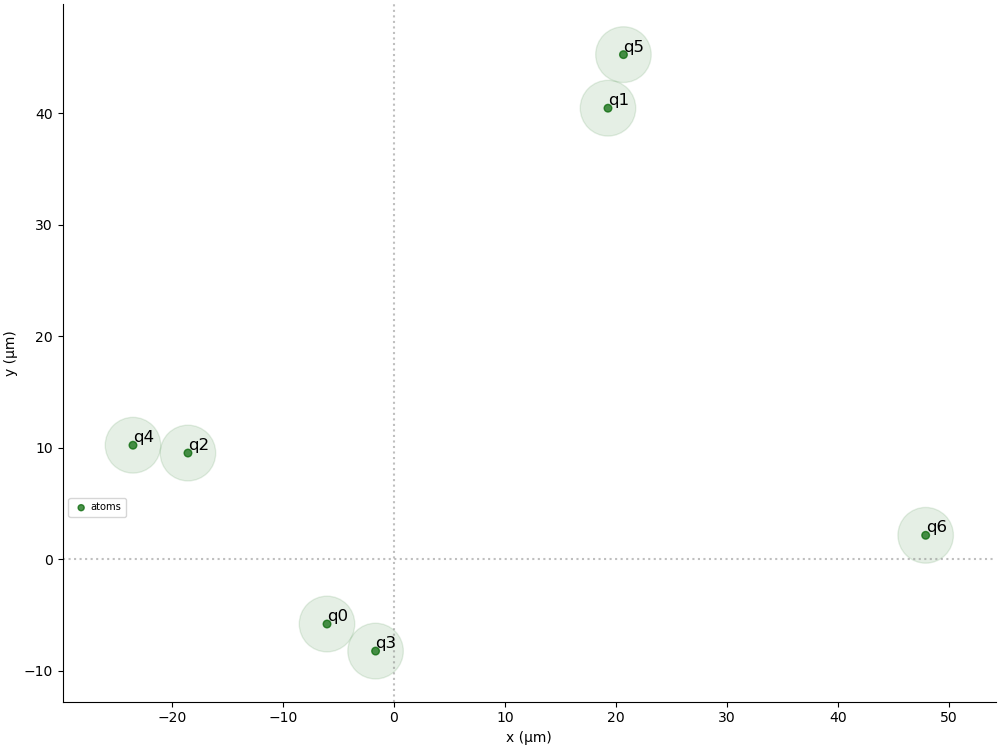
\includegraphics[width=0.8\textwidth]{img/embedding/reg_7x7.png} 
    \caption{The 2D physical spatial layout generated by the Genetic Algorithm for the $N=7$ instance. The register fully complies with Neutral Atom QPU geometric boundaries.}
    \label{fig:7x7_register}
\end{figure}

The physical layout reveals a highly structured and well-spaced geometric arrangement. Remarkably, the classical execution time was only $180.92$ seconds, achieving a very strong spatial fitness score of $2.266$. This excellent mathematical convergence set the expectation for an optimal quantum solution retrieval, which was subsequently confirmed by the QPU execution shown in Figure \ref{fig:7x7_quantum_res}.

\begin{figure}[htbp]
    \centering
    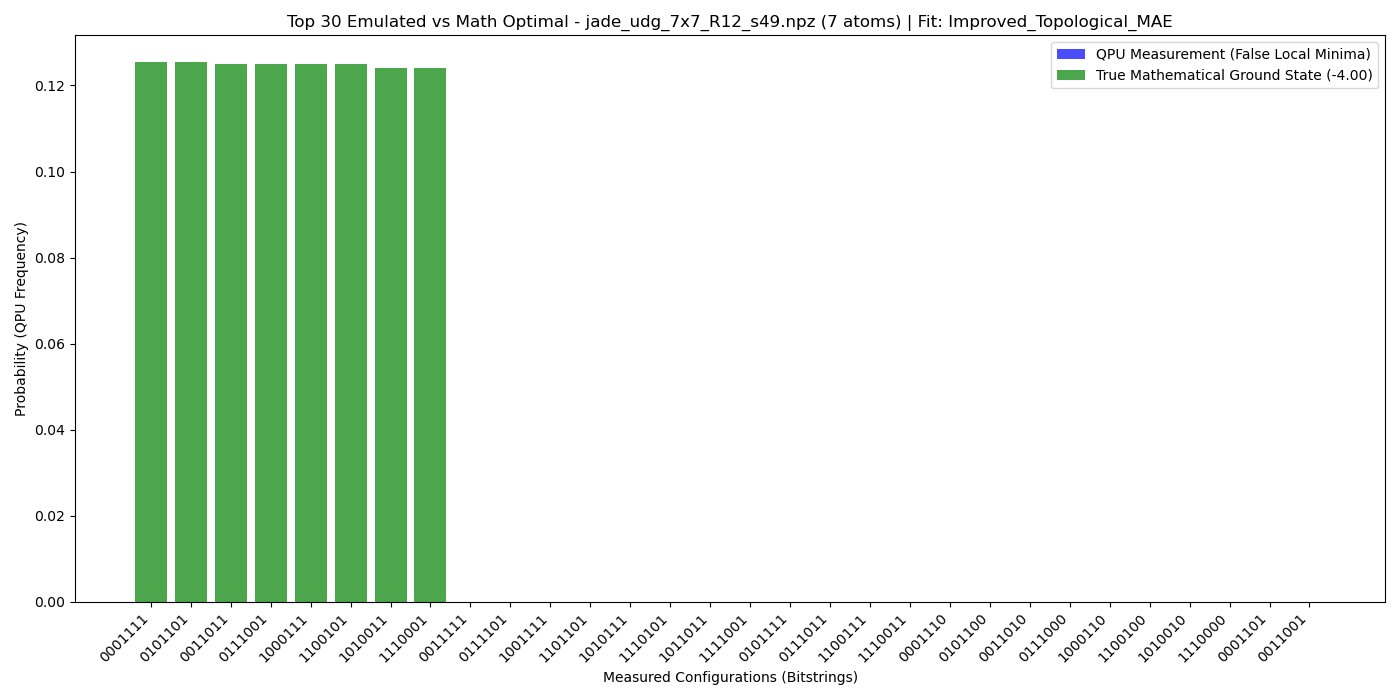
\includegraphics[width=1.0\textwidth]{img/res/res_7x7.png} 
    \caption{Probability distribution of the measured bitstrings after the adiabatic execution. The analog system successfully identifies the true mathematical ground states with a dominant probability mass, indicating a highly effective spatial embedding.}
    \label{fig:7x7_quantum_res}
\end{figure}

The quantum execution demonstrates perfectly symmetrical and outstanding results, effortlessly isolating the global optima. This instance is reported specifically to prove that the overall embedding difficulty is not dictated solely by the matrix dimensionality ($N$), but rather by a complex interplay of graph density, node degree distribution, and structural topology. Indeed, we observed that for this larger $7 \times 7$ grid, the hybrid pipeline obtained significantly better classical preprocessing times and quantum readout results than it did for the smaller, yet denser, $6 \times 6$ problem.

\section{10x10 instance}

\section{15x15 instance}




We have surely to consider that all the classical part has been executed on my laptop with the hardware specification in Appendix A \ref{app:hardware_specs}, with a better hardware and possibly a HP classical hardware capacity we would have been able, within the same execution time, to embed bigger matrices, but it is
however clear how in a "common" configuration of execution Genetic Algorithm imposes severe limitations in scalability. For this reasons other embedding methods has been studied and experimented and for the good results shown, Simulated Annealing will be presented in the following.



%continuare con le altre istanze che riteniamo valga la pena mostrare e con le modalità che riteniamo opportune.

%valutare quali istanze (le più rappresentative) andare a riportare spiegando bene e di nostro pugno
%i risultati ottenuti e le considerazioni relative al GA e le topologie delle istanze.


%Passare ad SA, spiegare perchè abbiamo usato SA perchè SA + GRASP (magari basta dire che degli esperimenti preliminari hanno giustificato l'uso di GRASP ecc ecc)
%Scegliere gli esperimenti più rappresentativi per SA + GRASP (magari qualcuno di confronto con GA e poi quelli che permettono di far vedere che si scala meglio), piccolo 
%confronto SA-SA + GRASP?

